\documentclass[english]{article}

\usepackage[latin9]{inputenc}
\usepackage[letterpaper]{geometry}
\geometry{verbose,tmargin=1in,bmargin=1in,lmargin=1in,rmargin=1in}
\usepackage{amsmath}
\usepackage{amssymb}
\usepackage{tikz}
\usetikzlibrary{automata,positioning}

\tikzstyle{dir}=[->, very thick]
\tikzstyle{circ}=[draw, circle, very thick]

\title{CIS 511 Homework 1}
\author{Stephen Phillips, Daegan Golomb}
\date{\today }


\begin{document}
\maketitle
\subsection*{Problem 1}

\subsubsection*{(c)}
Here the states $q_{ij}$ mean we have see $i$ (mod 2) $a$ symbols and $j$ b symbols (until 3 where we stop counting).

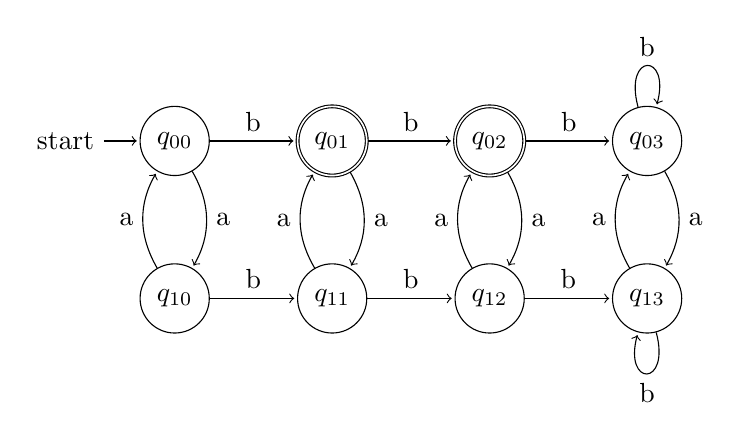
\begin{tikzpicture}[shorten >=1pt,node distance=2cm,on grid,auto] 
   \node[state,initial] (q_00)   {$q_{00}$}; 
   \node[state,accepting] (q_01) [right=of q_00] {$q_{01}$}; 
   \node[state,accepting] (q_02) [right=of q_01] {$q_{02}$};
   \node[state] (q_03) [right=of q_02] {$q_{03}$}; 
   \node[state](q_10) [below=of q_00] {$q_{10}$};
   \node[state](q_11) [right=of q_10] {$q_{11}$};
   \node[state](q_12) [right=of q_11] {$q_{12}$};
   \node[state](q_13) [right=of q_12] {$q_{13}$};
    \path[->] 
    (q_00) edge  node {b} (q_01)
          edge[bend left]  node  {a} (q_10)
    (q_01) edge  node {b} (q_02)
          edge[bend left]  node  {a} (q_11)
    (q_02) edge  node {b} (q_03)
          edge[bend left]  node  {a} (q_12)
    (q_03) edge [loop above] node {b} ()
          edge[bend left]  node {a} (q_13) 
    (q_10) edge  node {b} (q_11)
          edge[bend left]  node  {a} (q_00)
    (q_11) edge  node {b} (q_12)
          edge[bend left]  node  {a} (q_01)
    (q_12) edge  node {b} (q_13)
          edge[bend left]  node  {a} (q_02)
    (q_13) edge [loop below] node {b} ()
          edge[bend left]  node {a} (q_03);
\end{tikzpicture}

\subsubsection*{(g)}
Here the states $q_{ij}$ mean we have see $i$ (mod 2) total symbols and $j$ (mod 2) $a$ symbols. The top row is reversed to make the transitions more clear.

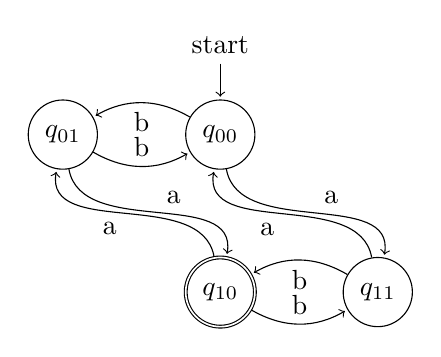
\begin{tikzpicture}[shorten >=1pt,node distance=2cm,on grid,auto] 
   \node[state,initial,initial where=above] (q_00)   {$q_{00}$}; 
   \node[state] (q_01) [left=of q_00] {$q_{01}$}; 
   \node[state,accepting](q_10) [below=of q_00] {$q_{10}$};
   \node[state](q_11) [right=of q_10] {$q_{11}$};
    \path[->] 
    (q_00) edge[bend right]  node {b} (q_01)
          edge[out=280,in=80]  node  {a} (q_11)
    (q_01) edge[bend right]  node {b} (q_00)
          edge[out=280,in=80]  node  {a} (q_10)
    (q_10) edge[bend right]  node {b} (q_11)
          edge[out=100,in=260]  node  {a} (q_01)
    (q_11) edge[bend right]  node {b} (q_10)
          edge[out=100,in=260]  node  {a} (q_00);
\end{tikzpicture}
%\begin{tikzpicture}[shorten >=1pt,node distance=2cm,on grid,auto] 
%   \node[state,initial] (q_0)   {$q_0$}; 
%   \node[state] (q_1) [above right=of q_0] {$q_1$}; 
%   \node[state] (q_2) [below right=of q_0] {$q_2$}; 
%   \node[state,accepting](q_3) [below right=of q_1] {$q_3$};
%    \path[->] 
%    (q_0) edge  node {0} (q_1)
%          edge  node [swap] {1} (q_2)
%    (q_1) edge  node  {1} (q_3)
%          edge [loop above] node {0} ()
%    (q_2) edge  node [swap] {0} (q_3) 
%          edge [loop below] node {1} ();
%\end{tikzpicture}

\subsection*{Problem 2}
\subsubsection*{(a)}
Using the method we did in class, we need to find $R_{ij}^k$ for $i,j \in \{0,1,2\}, k \in \{1,2\}$. The general formula is
$ R_{i,j}^{k+1} = R_{i,j}^{k} \cup (R_{i,k+1}^{k} (R_{k+1,k+1}^{k})^{*}) R_{k+1,j}^{k} $. For brevity any $\varepsilon$ inside a kleene star, as that is given.
\begin{align*}
R_{11}^{0} &=\; a\cup\varepsilon \\
R_{12}^{0} &=\; b \\
R_{21}^{0} &=\; b \\
R_{22}^{0} &=\; a\cup\varepsilon \\
R_{11}^{1} &=\; R_{11}^0 \cup R_{11}^0 R_{11}^{0*} R_{11}^0 = a\cup\varepsilon \cup ((a\cup\varepsilon) a^{*} (a\cup\varepsilon)) \\
R_{12}^{1} &=\; R_{12}^0 \cup R_{11}^0 R_{11}^{0*} R_{12}^0 = b \cup ((a\cup\varepsilon) a^{*} b) \\
R_{21}^{1} &=\; R_{21}^0 \cup R_{21}^0 R_{11}^{0*} R_{11}^0 = b \cup (b a^{*} (a\cup\varepsilon)) \\
R_{22}^{1} &=\; R_{22}^0 \cup R_{21}^0 R_{11}^{0*} R_{12}^0 = a\cup\varepsilon \cup (b a^{*} b) \\
R_{12}^{2} &=\; R_{12}^1 \cup R_{12}^1 R_{22}^{1*} R_{22}^1 = (b \cup (a\cup\varepsilon) a^{*} b) \cup ((b \cup ((a\cup\varepsilon) a^{*} b)) (a\cup\varepsilon \cup b a^{*} b)^{*} (a\cup\varepsilon \cup (b a^{*} b))) \\
\end{align*}
So the final regular expression is $R_{12}^{2} = (b \cup (a\cup\varepsilon) a^{*} b) \cup ((b \cup ((a\cup\varepsilon) a^{*} b)) (a\cup\varepsilon \cup b a^{*} b)^{*} (a\cup\varepsilon \cup (b a^{*} b)))$. The simpler regular expression is $a^{*} b a^{*} (b a^{*} b a^{*})^{*}$ (seen from inspection), gives the same thing.

\subsubsection*{(b)}
We again use the same technique, this time in tabular form. The general formula is, again, 
$ R_{i,j}^{k+1} = R_{i,j}^{k} \cup (R_{i,k+1}^{k} (R_{k+1,k+1}^{k})^{*}) R_{k+1,j}^{k} $. For brevity any $\varepsilon$ inside a kleene star, as that is given.

\begin{table}[h]
\begin{tabular}{c|c|c|c|c}
$R_{ij}$/Level & 0                & 1                    & 2                            & 3 \\
$R_{11}$       &$\varepsilon$     &$\varepsilon$         &$\varepsilon$            &$\varepsilon\cup(a\cup b)a^*b(ba^*b)^*a$  \\
$R_{12}$       &$a \cup b$        &$a \cup b$            &$(a\cup b)\cup(a\cup b)a^*a$  &(Not ending on final state)  \\
$R_{13}$       &$\varnothing$     &$\varepsilon$         &$(a\cup b)a^*b$               &$(a\cup b)a^*b\cup(a\cup b)a^*b(ba^*b)^*ba^*b$  \\
$R_{21}$       &$\varnothing$     &$\varnothing$         &$\varnothing$                 &(Not starting at initial state) \\
$R_{22}$       &$a\cup\varepsilon$&$a\cup\varepsilon$    &$a\cup\varepsilon\cup (a\cup\varepsilon)a^*(a\cup\varepsilon)$  &(Not starting at initial state) \\
$R_{23}$       &$b$               &$b$                   &$b\cup (a\cup\varepsilon)a^*b$                 &(Not starting at initial state) \\
$R_{31}$       &$a$               &$a$                   &$a$                           &(Not starting at initial state) \\
$R_{32}$       &$b$               &$b \cup (b(a \cup b))$&$b\cup b(a\cup b)\cup((b\cup b(a\cup b))a^*(a\cup\varepsilon)$&(Not starting at initial state) \\
$R_{33}$       &$\varepsilon$     &$\varepsilon$         &$ba^*b$                     &(Not starting at initial state)  
\end{tabular}
\end{table}

So the final expression is $ R_{11}^{3} \cup R_{13}^{3} = ((\varepsilon\cup(a\cup b)a^*b(ba^*b)^*a) \cup ((a\cup b)a^*b\cup(a\cup b)a^*b(ba^*b)^*ba^*b) $. This
DFA does not have any intuitive regular expression that can be seen from inspection, so this technique is the best way to do it.

\subsection*{Problem 3}
Claim: If a language $A$ is regular, then its reverse $A^\mathcal{R}$ is regular.
Proof:
Let $M = (Q,\Sigma,\delta,q_0,F)$ be the DFA accepting the language $A$. Create the NFA $N = (Q',\Sigma,\delta',q_0',F')$. The idea is to make $N$ such that it reverses all the edges of $M$, and create a new start state that has epsilon transitions to the final states of $M$, with the accepting state being the starting state of $M$. Specifically:
\begin{align*}
                           Q' &=\; Q \cup \{q_0'\} \\
 \delta(q \in Q,a \in \Sigma) &=\; \{ q' \in Q | \delta(q',a) = q \} \\
        \delta(q_0',\epsilon) &=\; F \\
                           F' &=\; \{q_0\}
\end{align*}

All transitions not specified map to the empty set. Now we have to show this machine accepts a string if and only if the string is in $A^\mathcal{R}$.

Proving that it accepts if the string is in $A^\mathcal{R}$ is rather simple. If a string $s \in A^\mathcal{R}$ then there is a path from one of the final paths to the initial state of $M$, since the reverse of the string would have been accepted by $M$. Therefore our machine $N$ accepts this string.

Now we must prove it does not accept any other strings. Suppose not, and there was a string $s \notin A^\mathcal{R}$ that was accepted by this machine. Since it accepted, there must have been at least one path to the initial state of $M$. However, we started at all the final states of $M$, since our initial state $q_0'$ only had epsilon transitions to the final states of $M$, and went to nothing else. So that means there is a path from a final state to the initial state. There cannot be more than one of these paths because $M$ was a DFA. This means that the reverse of this string would have been accepted $M$, which is a contradiction since we assumed that $s \notin A^\mathcal{R}$.

We have proved this machine $N$ accepts only strings in $A^\mathcal{R}$. Since any NFA can be converted to a DFA, that means $A^\mathcal{R}$ is regular for any regular language $A$.

\subsection*{Problem 4}
So an all-NFA $M$ is a five-tuple $(\Sigma,Q,\delta,q_0,F)$, that acts just like an NFA except it only accepts if all non-deterministic paths end up in states in $F$. We will show that this recognizes the set of regular languages.

In one direction, any DFA is an all-NFA. Since in a DFA's $\delta$ only maps a state to only one other state, we only ever have one path, and therefore if a string gives an accepting path, the final state it ends up in is the only final state it ends up in (you know, determinism).

In the other direction, we can create a DFA for any all-NFA. It is similar to the construction of DFA's for normal NFAs. So, given an all-NFA $M = (\Sigma,Q_M,\delta_M,q_{M0},F_M)$, we can construct DFA $N = (\Sigma,Q_N,\delta_N,q_{N0},F_N)$. For completeness, let the function $\mathcal{N}_\varepsilon(S)$ denote the 'epsilon closure' as described in the book - the set of all nodes in $S$ and reachable by $S$ via epsilon transitions.

\begin{align*}
                              Q_N &=\; \mathbb{P}(Q_M) \\
 \delta_M(q \in Q_N,a \in \Sigma) &=\; \{ q' \in Q_M | q' \in \mathcal{N}_\varepsilon(\delta(q,a)) \} \\
                           q_{N0} &=\; \{q_{M0}\} \\
                              F_N &=\; \{ S | S \subseteq F_M \} \\
\end{align*}

The proof is, again, very similar to the proof that NFAs recognize regular languages. This machine works exactly as an NFA, which as was shown in the book. The only difference is that the accepting states are those subsets of $Q_M$ that have only members in the final states of $M$, $F_M$. This exactly satisfies the conditions for an all-NFA.

Therefore, the set of languages that all-NFAs accept is the set of regular languages.

\subsection*{Problem 5}
Let $A$ be a language over $\{0,1\}^*$. Define the language $B$ called even-$A$ as follows:
\[ B = \{ v_1 v_2 \cdots v_k | \exists w_1 w_2 \cdots w_k : w_1 v_1 w_2 v_2 \cdots w_k v_k \in A \} \]
Prove $B$ is regular.

Consider the DFA $M = (\Sigma,Q_M,\delta_M,q_{M0},F_M)$. Create a new NFA $N = (\Sigma,Q_N,\delta_N,q_{N0},F_N)$ that accepts $B$ using $A$. The idea is to skip every other state. In other picture form, this:

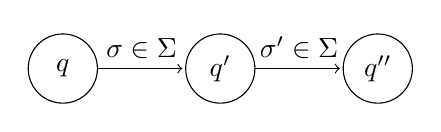
\begin{tikzpicture}[shorten >=1pt,node distance=2cm,on grid,auto] 
   \node[state] (q_00)   {$q$}; 
   \node[state] (q_01) [right=of q_00] {$q'$}; 
   \node[state] (q_10) [right=of q_01] {$q''$};
    \path[->] 
    (q_00) edge node {$\sigma \in \Sigma$}  (q_01)
    (q_01) edge node {$\sigma' \in \Sigma$} (q_10);
\end{tikzpicture}

Turns into this:

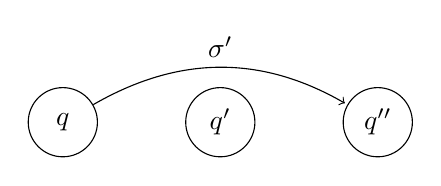
\begin{tikzpicture}[shorten >=1pt,node distance=2cm,on grid,auto] 
   \node[state] (q_00)   {$q$}; 
   \node[state] (q_01) [right=of q_00] {$q'$}; 
   \node[state] (q_10) [right=of q_01] {$q''$};
    \path[->] 
    (q_00) edge[bend left] node {$\sigma'$}  (q_10);
\end{tikzpicture}

More formally:
\begin{align*}
                              Q_N &=\; Q_M \\
 \delta_M(q \in Q_N,a \in \Sigma) &=\; \{ q' \in Q_M | \exists b \in \Sigma : q' = \delta(\delta(q,b),a) \} \\
                           q_{N0} &=\; \{q_{M0}\} \\
                              F_N &=\; F_M \\
\end{align*}

Now we show this only accepts strings in $B$. 

This comes by construction as we skip every other transition. Therefore, to construct a string in $A$, we take the accepting path and insert the symbols we skipped, and therefore we have a string in $B$. So if a string is accepted we can find a string in $A$ that it corresponds to. And it cannot accept any string not in $B$ since we can construct this string from $A$. 

\subsection*{Problem 6}
Let $A/B = \{w|wx \in A \text{ for some } x \in B\}$. Show that if $A$ is regular and $B$ is any language, then $A/B$ is regular.

Once we view this properly, the solution is intuitive. The idea is to include any state that could lead from $w$ into $x$ for some $x \in B$ and include it in the list of possible final states. In other words, we accept any string that is $w$ after we have removed some word from $B$. Note that this simple solution does not assume that iterating through all removals of $B$ to build this DFA is easy.

\subsection*{Problem 7}
\subsubsection*{(a)}
Let $L = \{0^n 1^m 0^n | m,n \geq 0\}$. Let $p$ be the pumping lemma constant. Construct $s = 0^p 1 0^p$.
Note $s \in L$ and let $s = xyz$ as given by the pumping lemma.
Since $|xy| \leq p$, $y$ consists of only $0$'s. Choose $w = xy^2 z$, i.e., choose $i=2$. This has strictly more than $p$ zeros on the left and exactly $p$ zeros on the right. Thus, $w \notin L$ and hence, by contraction of PL, $s$ cannot be regular. This is a contradiction.

\subsubsection*{(c)}
Let $L = \{w|w \in \{0,1\}^* \text{ is not a palindrome}\}$. By closure over the set of regular languages, the complement of $L$, $L' = \{w|w \in \{0,1\}^* \text{ is a palindrome}\}$, must also be regular. We will prove $L'$ is not regular and hence, neither is $L$:\\
Let $p$ be the pumping lemma constant. Construct $s = 0^p 1^p$.
Note $s \in L$ and let $s = xyz$ as given by the pumping lemma.
Since $|xy| \leq p$, $y$ consists of only $0$'s. Choose $w = xy^2 z$, i.e., choose $i=2$. This has strictly more than $p$ zeros (on the left) and exactly $p$ ones (on the right). Thus, $w$ cannot be a palindrome and therefore $w \notin L'$ and hence, by contraction of PL, $s$ cannot be regular. This is a contradiction.\\
By contradiction of its complement the original claim holds.

\subsection*{Problem 8}
Claim: The relation $x \equiv_L y$, meaning $\forall z \in \{0,1\}^*, xz \in L \iff yz \in L$, is an equivalence relation.
\begin{itemize}
\item Reflexivity: Obviously $x$ is indistinguishable from $x$, since $\forall z \in \{0,1\}^*, xz = xz \implies xz \in L \iff zz \in L$.
\item Symmetry: This follows from the if and only if of the definition of $\equiv_L$, which is itself is an equivalence relation. Meaning $(xz \in L \iff yz \in L) \iff (yz \in L \iff xz \in L)$
\item Transitivity: This also follows from the if and only if of the definition. Suppose $\equiv_L$ was not transitive, then there are strings $x,y,w$ such that $\forall z' \in \{0,1\}^*, xz' \in L \iff yz' \in L$ and $yz \in L \iff wz \in L$ but $\exists z \in \{0,1\}^* xz \in L, wz \notin L$. However, we know that if $wz \notin L$, then $yz \notin L$, and if $yz \notin L$ then $xz \notin L$. This is a contradiction, saying $xz$ is both in $L$ and not in $L$. Therefore this relation is transitive.
\end{itemize}

We have shown all properties of an equivalence relation, so $x \equiv_L y$ is an equivalence relation.

\subsection*{Problem 9}
We construct the new automaton by simulating the two original ones simultaneously:\\
Let $M_1 = <Q_1, q_{0_1}, \Sigma_1, \delta_1, F_1>$ and $M_2 = <Q_2, q_{0_2}, \Sigma_2, \delta_2, F_2>$.\\
Construct $M = <Q_1 \times Q_2, (q_{0_1}, q_{0_2}), \Sigma_1 \cup \Sigma_2, \delta = \{\{(a,b), (c,d)\}|(a,c) \in \delta_1 \text{ and } (b,d) \in \delta_2\}, F_1 \times F_2>$.\\
Now, if $L_1$ accepts a string, then there exists paths that traverse from $q_{0_1}$ to a state in $F_1$. The similar holds for the second element with regards to $L_2$. The only way to traverse from $(q_{0_1}, q_{0_2})$ to an element in $F_1 \times F_2$ is to traverse on each field of the tuple. Therefore, this DFA only accepts strings that satisfies both original DFAs. Thus, this DFA accepts $L_1 \cap L_2$.

\end{document}
